\documentclass{article}
\usepackage[utf8]{inputenc}

% Standard packages that I use for math documents.
\usepackage[margin=0.75in]{geometry}
\usepackage{enumerate}
\usepackage{amsmath}
\usepackage{amsfonts} 
\usepackage{amssymb}
\usepackage{amsthm}
\usepackage{mathtools}
\usepackage{float}
\usepackage{array}
\usepackage{makecell}
\usepackage{commath}
\usepackage{easybmat} % for block matrices
\usepackage{parskip}
% Document-specific packages
\usepackage{xcolor, soul} % for highlights
\sethlcolor{yellow}

% Standard settings I use for nice formatting.
\setlength\parindent{0pt}
\DeclarePairedDelimiter{\ceil}{\lceil}{\rceil}
\renewcommand\theadalign{bc}
\renewcommand\theadfont{\bfseries}
\renewcommand\theadgape{\Gape[4pt]}
\renewcommand\cellgape{\Gape[4pt]}

% Standard definitions of macros I use regularly.
\newcommand{\N}{\mathbb{N}}
\newcommand{\Z}{\mathbb{Z}}
\newcommand{\Q}{\mathbb{Q}}
\newcommand{\C}{\mathbb{C}}
\newcommand{\R}{\mathbb{R}}
\newcommand{\F}{\mathbb{F}}
\newtheorem{theorem}{Theorem}
\newtheorem{proposition}{Proposition}[section]
\newtheorem{hypothesis}{Hypothesis}[section]
\newtheorem{corollary}{Corollary}[theorem]
\newtheorem{definition}{Definition}[section]
\newtheorem{lemma}[theorem]{Lemma}
\newtheorem*{remark}{Remark}
\newcommand{\cdotscalar}{\;\widetilde{\cdot}\;}
\newcommand{\vectorplus}{\;\widetilde{+}\;}
\newcommand{\Span}{\text{Span}}
\newcommand{\Null}{\text{Null}}
\newcommand{\Range}{\text{Range}}
\newcommand{\D}{\frac{d}{\dif x}}
\renewcommand{\epsilon}{\varepsilon}
\newcommand{\Or}{\mbox{ OR }}
\renewcommand{\And}{\mbox{ AND }}
\newcommand{\Not}{\mbox{NOT }}
\newcommand{\Iff}{\mbox{ IFF }}
\newcommand{\Width}{\textup{width}}
\newcommand{\Mesh}{\textup{mesh}}
\newcommand{\Int}{\textup{Int}}
\newcommand{\Ext}{\textup{Ext}}
\newcommand{\Bd}{\textup{Bd}}
\newcommand{\Supp}{\textup{Support}}
\newcommand{\sgn}{\textup{sgn}}
\newcommand{\loss}{\textup{loss}}
\newcommand{\insamplegeqx}{\textup{\texttt{insample$\geq$x}}}
\newcommand{\insampleltx}{\textup{\texttt{insample$<$x}}}
\newcommand{\insample}{\textup{\texttt{insample}}}
\newcommand\widebar[1]{\mathop{\overline{#1}}}
\newcommand*\closure[1]{\widebar{#1}}
\newcommand\Ball[2]{U(#1; #2)}

\newcommand{\1}{\langle 1 \rangle}
\newcommand{\2}{\langle 2 \rangle}

% End of preamble.  

\begin{document}

\tableofcontents

\section{Some notes from which to expand this document}

\begin{enumerate}
    \item An overview of coupling proofs of privacy
    \item A tight shift-coupling proof of privacy (segment free)
    \begin{enumerate}
        \item What are the connecting constraints, and why are they there?
        \item Proofs have to depend on $\Delta$!
        \item Proofs have to depend on sequences of segments! 
    \end{enumerate}
    \item Simplifying the problem above in various ways: 
    \begin{enumerate}
        \item Separability and the introduction of segments
        \item Only inter-segment transitions matter! 
        \begin{itemize}
            \item Given $\Delta$, the $\gamma$ values on inter-segment transitions are easily determined. 
            \item The $\Delta$ values on the inter-segment transitions can be determined. 
        \end{itemize}
    \end{enumerate}
    \item Solving the problem.
    \begin{enumerate}
        \item Hardness (incomplete)!!!
        \item Solving the easier version, where proofs don't depend on $\Delta$.
        \item Showing that they are bounded within $n$ of each other. 
        \begin{align*}
            \exists \text{ finite DP bound } &\iff \text{ hard system admits a feasible solution }
        \end{align*}
    \end{enumerate}
\end{enumerate}

\section{Definitions}

\subsection{DiPA}

Insert definition for DiPA here. 

\subsection{Probability}

\begin{definition}
    The probability $\Pr(\rho | X)$ of a path $\rho = q_0 \to q_1 \to \dots \to q_m$ given an input $X = \langle a_1 , \dots, a_m \rangle$ is defined recursively as the probability that all transitions in $\rho$ are traversed in sequence given the input $X$ starting at state $q_0$.
\end{definition}

\begin{definition}
    Let $\mathcal{A}$ be a DiPA, and $s \in seg(\mathcal{A})$ be a segment. The \textbf{privacy loss} $\loss(s)$ of a segment $s \in seg(\mathcal{A})$ is defined as 

    \[\loss(s) = \sup_{\rho \in segF(s)}\sup_{X' \sim X} \left(\frac{Pr(\rho | X)}{P(\rho | X')} \right) \]

    where $X$ and $X'$ vary over all pairs of neighbouring datasets. 
\end{definition}

\begin{definition}
    Let $f_\epsilon(x)$ be the probability density function of a random variable $X$ with $X \sim Lap(0, 1/\epsilon)$. 

    \[f_\epsilon(x) = \frac{\epsilon}{2} \exp(-\epsilon |x|)\]
\end{definition}

\begin{definition}
    Let $F_\epsilon(x)$ be the cumulative distribution function of a random variable $X$ with $X \sim Lap(0, 1/\epsilon)$.

    \[F_\epsilon(x) = P(X \leq x) = \begin{cases}
        \frac{1}{2} \exp(\epsilon x) & x < 0 \\
        1 - \frac{1}{2} \exp(-\epsilon x) & x \geq 0
    \end{cases}\]
\end{definition}

\newpage
\section{Coupling proofs of privacy}

A coupling proof of privacy 

\newpage
\section{Shift-coupling proofs of privacy}

Consider a path $\rho = q_0 \to q_1 \to \dots \to q_m$. Consider inputs $X \langle 1 \rangle = \langle a_1 \langle 1 \rangle, \dots, a_m \langle 1 \rangle \rangle$ and $X \langle 2 \rangle = \langle a_1 \langle 2 \rangle, \dots, a_m \langle 2 \rangle \rangle$ such that $X \langle 1 \rangle \sim X \langle 2 \rangle$. We wish to show that there exists $\epsilon \in (0, \infty)$ such that

\begin{align*}
    \Pr\left[\rho | X \langle 1 \rangle \right] \leq \exp(\epsilon) \cdot \Pr\left[\rho | X \langle 2 \rangle\right]
\end{align*}

\hl{TODO}: Write all of this later after consulting with Sky! ALSO, distinguish between path equivalence and output equivalence.

\begin{definition}
    Let  $X = \langle a_1, \dots, a_m \rangle$ be an input, and $\rho = q_0 \to q_1 \to \dots \to q_m$ be a path taken by DiPA $\mathcal{A}$ on $X$. Define $\tilde{a_i}$ to be the value of $\insample$ on the $i$th transition in $\rho$ on input $X$.
\end{definition}

\begin{itemize}
    \item The above is true if and only if $path_A(X) \Psi_\rho^{(\epsilon, 0)} path_A(X')$, where

    \[\Psi_\rho = \{(\rho_1, \rho_2) \in P \times P : \rho_1 = \rho \implies \rho_2 = \rho \} \]
    
    Shift-couplings are a technique to show that $path_A(X) \Psi_\rho^{(\epsilon, 0)} path_A(X')$ by constructing the couplings
    
    \[\tilde{a_i} \1 + \gamma_i (=)^{\#(\epsilon_i, 0)} \tilde{a_i} \2 \qquad \forall i \in \{0, \dots, m - 1\}\]

    and showing that 

    \[(\tilde{a} \1 + \gamma = \tilde{a} \2) \implies path_A(X \1) \Psi_\rho path_A(X \2)\]

    thus showing that $path_A(X) \Psi_\rho^{(\epsilon, 0)} path_A(X')$ for \[\epsilon = \sum_{i = 0}^{m - 1} \epsilon_i\]
    
    % where \[\psi_{\rho, i} = \{(\rho_1, \rho_2) \in P \times P : \rho_1[i] = \rho[i] \implies \rho_2[i] = \rho[i]\}\]
    
    % \[A(X) \Psi_{o, i} A(X') \qquad \forall i \in \{1, \dots, m\}\] where 
    \item A discussion that ends in choosing $\gamma$ shifts for each segment. 
    \item Maybe: A discussion of the cost of each shift.    
\end{itemize}


\subsection{Connecting constraints} 

\begin{definition}
    
Given a fixed path, we say that an assignment of shifts $\{\gamma_i\}$ is \textbf{valid} if

\[(\tilde{a} \1 + \gamma = \tilde{a} \2) \implies path_A(X \1) \Psi_\rho path_A(X \2)\]

\end{definition}

\begin{definition}
    Let $\rho = q_0 \to q_1 \to \dots \to q_m$ be a path, and let $i \in \{1, \dots, m\}$. Define $at(i)$ to be the largest index $a(i) < i$ such that $\rho[a(i)] \to \rho[a(i) + 1]$ is an assignment transition.  
\end{definition}

\begin{definition}
    Let $\rho = q_0 \to q_1 \to \dots \to q_m$ be a path. Define $t_i$ to be the transition $q_i \to q_{i + 1}$.
\end{definition}

\begin{definition}
    Let $X = \langle a_1, \dots, a_m \rangle$ be an input, and let $\rho = q_0 \to q_1 \to \dots \to q_m$ be a path. Define $X[i]$ to be the value of $a_i$.
\end{definition}

Note that such an index must exist due to the initialization condition on DiPA. 

\begin{proposition}
    Given $\rho = q_0 \to q_1 \to \dots \to q_m$, an assignment of shifts $\{\gamma_i\}$ is valid if and only if it satisfies the following constraints for all $i \in \{0, \dots, m - 1\}$:

    \begin{align*}
        \gamma_i \leq \gamma_{at(i)} \qquad &\text{if } t_i \text{ has guard } < \\
        \gamma_i \geq \gamma_{at(i)} \qquad &\text{if } t_i \text{ has guard } \geq \\
    \end{align*}
\end{proposition}

\begin{proof}
    (Constraints $\implies$ valid) Suppose that the above constraints hold. We will show that $\{\gamma_i\}$ is valid using induction on $m = |\rho|$. Construct the couplings $\tilde{a_i} \1 + \gamma_i (=)^{(\epsilon_i, 0)} \tilde{a_i} \2$ for all $i \in \{0, \dots, m - 1\}$. 

    For a base case, assume $m = 1$. Then $\rho$ consists of an assignment transition $t_0$ with \texttt{true} guard (initialization condition). The constraints are trivially satisfied, and we have that $path_A(X \1 ) \Psi_\rho^{(0, 0)} path_A(X \2)$.

    Assume that the constraints hold for all paths of length $m$. Let $\rho = q_0 \to q_1 \to \dots \to q_{m} \to q_{m + 1}$. We will show that $\{\gamma_i\}$ is valid for $\rho$. First, by the validity of $\{\gamma_i\}_{i = 0}^{m - 1}$ for $\rho[0:m]$ by the inductive hypothesis, we have that \[path_A(X \1) \Psi_{\rho[0:m]} path_A(X \2)\] 
    
    by the inductive hypothesis. Now, assume $path_A(X \1) = \rho$. We have $path_A(X \2)[0:m] = \rho[0:m]$. Consider the last transition $t_{m}$ in $\rho$. Since $path_A(X \1) = \rho$, we know that $t_m$ is traversed by $A$ on $X \1$.

    \begin{itemize}
        \item If $t_{m}$ has guard \texttt{true}, then we trivially have that $path_A(X \2) = \rho$.
        \item If $t_{m}$ has guard $<$, we have from the constraints that $\gamma_{m} \leq \gamma_{at(m)}$. The value of the state variable $x \langle 1 \rangle$ is 
        
        \[x \1 = \tilde{a}_{at(m)} \1 \]

        and since $t_m$ is traversed by $A$ on $X \1$, we have 

        \begin{align*}
            \tilde{a}_{m} \1 &< \tilde{a}_{at(m)} \1\\
            \tilde{a}_{m} \2 - \gamma_m &< \tilde{a}_{at(m)} \2 - \gamma_{at(m)}\\
            \tilde{a}_{m} \2 &< \tilde{a}_{at(m)} \2 - (\gamma_{at(m)} - \gamma_{m}) < \tilde{a}_{at(m)} \2\\
        \end{align*}

        showing that $\tilde{a}_{m} \2$ satisfies the guard of $t_m$. Thus, $path_A(X \2) = \rho$.
        \item If $t_{m}$ has guard $\geq$, a similar argument as above shows that $path_A(X \2) = \rho$.
    \end{itemize}

    Thus, assuming that $a \1 + \gamma = a \2$, we have shown that $path_A(X \1) = \rho \implies path_A(X \2) = \rho$, which shows $path_A(X \1) \Psi_\rho path_A(X \2)$, and so $\{\gamma_i\}$ is valid.

    (Valid $\implies$ constraints) Suppose that $\{\gamma_i\}$ is valid. Let $i \in \{0, \dots, m - 1\}$. We will show that the constraints hold for $i$. 

    We will run the argument above in reverse. Again, we use induction on the length $m = |\rho|$. For a base case, assume $m = 1$, and so $\rho$ consists of an assignment transition $t_0$ with \texttt{true} guard. The constraints are trivially satisfied, since there are none. 

    Assume that the constraints hold for all valid shift assignments on paths of length $m$, and let $\rho = q_0 \to q_1 \to \dots \to q_{m} \to q_{m + 1}$. Since $\{\gamma_i\}$ is valid for $\rho$, we have that $a \1 + \gamma = a \2 \implies path_A(X \1) \Psi_\rho path_A(X \2)$. Also, we have that $\{\gamma_i\}_{i = 0}^{m - 1}$ is valid for $\rho[0:m]$, and that constraints on transitions $t_i \in \rho[0:m]$ hold. 

    We will now show that the constraints on $t_{m}$ hold by cases on the guard of $t_{m}$.

    \begin{itemize}
        \item If $t_{m}$ has guard \texttt{true}, then there is no constraint on $\gamma_{m}$, and so the constraints hold.
        \item If $t_{m}$ has guard $<$, the constraint to be shown is $\gamma_m \leq \gamma_{at(m)}$. Recall that we have $a \1 + \gamma = a \2 \implies path_A(X \1) \Psi_\rho path_A(X \2)$, showing that $t_m$ being traversed by $A$ on $X \1$ leads $t_m$ to be traversed by $A$ on $X \2$. Thus, we have 
        
        \begin{align*}
            \tilde{a}_m \1 < \tilde{a}_{at(m)} \1 &\implies \tilde{a}_m \2 < \tilde{a}_{at(m)} \2\\
             &\iff \tilde{a}_m \1 + \gamma_m < \tilde{a}_{at(m)} \1 + \gamma_{at(m)}\\
             &\iff \tilde{a}_m \1 < \tilde{a}_{at(m)} \1 + (\gamma_{at(m)} - \gamma_m)\\
        \end{align*}

        which is true if and only if $\gamma_m \leq \gamma_{at(m)}$. Thus, the constraint holds.
        \item A symmetric argument shows that the constraint holds if $t_{m}$ has guard $\geq$.
    \end{itemize}

    Thus, the given constraints on $\gamma$ hold if and only if it is valid for $\rho$.
\end{proof}

\begin{theorem}
    A choice of valid $\{\gamma_i\}$ for each path $\rho$ and pairs of inputs $X \1 \sim X\2$ which satisfies 
    \begin{align*}
        \gamma_i = 0 \qquad &\text{if } t_i \text{ outputs \texttt{insample} or \texttt{insample'}} 
    \end{align*} 
    shows that $\mathcal{A}$ is $(\epsilon, 0)$-differentially private, where $\epsilon = \sup_{X \1 \sim X \2} \sup_{\rho} cost(\{\gamma_i\})$. TODO: Define cost. Maybe prove a proposition before this about (path equivalence and output constraints) $\iff$ output equivalence.
\end{theorem}

\begin{proof}
    By definition, almost. 
\end{proof}

\subsection{The cost of a shift-coupling}

\begin{proposition}
    Consider a transition $t_i = q_{i} \to q_{i + 1}$ which is traversed independently by $A$ on input $a_i \1$ and $a_i \2$. Let $\Delta_i = a_i \2 - a_i \1$. Let $q_i$ draw from the distribution $Lap(0, \epsilon_i)$ to noise \texttt{insample}. The $\epsilon$-cost of the shift-coupling 

    \[\tilde{a_i} \1 + \gamma_i (=)^{(c_i, 0)} \tilde{a_i} \2\]

    is given by \[c_i = |\Delta_i - \gamma_i| \epsilon_i \]
\end{proposition} 

\begin{proof}
    TODO
\end{proof}

\subsection{A tight proof must regard input differences}

Since the total validity constraints on $\{\gamma_i\}$ does not depend on $X \1$ and $X \2$, one might be tempted to produce a proof of privacy by choosing $\gamma_i$ to be the same for all $X \1$ and $X \2$, given a path $\rho$. Although this is possible, this does not in general produce a tight proof of privacy.

\begin{proposition}
    
\end{proposition}

\subsection{A tight proof must regard paths}

\section{The search for a tight proof as an optimization problem}

\subsection{Leading upto the abstract formulation}

\subsection{The problem as a whole}


\subsection{Specifying the inner minimization problem}

Here, we specify how $A_{s, \boldsymbol{\Delta}}$ and $c_{s, \boldsymbol{\Delta}}$ are defined. Let $s = s_1 \hookrightarrow \dots \hookrightarrow s_n$ be a sequence of segments with total number of transitions $m$. Let $\boldsymbol{\Delta} \in \{-1, 0, 1\}^m$ be a vector of input perturbations.

We define some notation as follows: 

\begin{itemize}
    \item Let $t^i_j$ denote the $j$th transition in segment $i$, and $\epsilon^i_j$ denote the noise added to the input before that transition.
    \item Let $\Delta^i_j$ denote the entry of $\boldsymbol{\Delta}$ that corresponds to the input perturbation for the $j$th transition in segment $i$.
    \item Let $\gamma^i_j$ denote the entry of $\boldsymbol{\gamma} \in [-1, 1]^m$ that corresponds to the coupling shift for the $j$th transition in segment $i$ -- this is to be determined by the inner minimization problem.
\end{itemize}

Then, the minimization problem over $\boldsymbol{\gamma}$ is as follows:

\begin{align*}
\min_{\boldsymbol{\gamma} \in [-1, 1]^m} \quad & \sum_{i = 1}^n \sum_{j = 1}^{|s_i|} |\gamma^i_j - \Delta^i_j| \epsilon_i \\[2em]
\text{subject to } \quad 
& \gamma^i_k \leq \gamma^i_0 &\text{if $t^i_k$ has guard $<$} \\
& \gamma^i_k \geq \gamma^i_0 &\text{if $t^i_k$ has guard $\geq$} 
\\[1em]
& \gamma^i_0 \leq \gamma_0^k &\text{if $s_k \hookrightarrow s_i$ and guard($s_i$) is $<$} \\
& \gamma^i_0 \geq \gamma_0^k &\text{if $s_k \hookrightarrow s_i$ and guard($s_i$) is $\geq$} 
\\[1em]
& \gamma^i_k = 0 &\text{if $t^i_k$ outputs \texttt{insample}} \\
& \gamma^i_k = \Delta^i_k &\text{if $t^i_k$ belongs to a cycle} 
\end{align*}

This can be rewritten as a linear program using standard techniques, producing a constraint matrix $A_{s, \boldsymbol{\Delta}}$ and a cost vector $c_{s, \boldsymbol{\Delta}}$.

\subsection{A simplification}

Let $\mathcal{F}$ be a finite family of segment sequences. The global optimization problem is to find 

\begin{align*}
\max_{s \in \mathcal{F}} \max_{\boldsymbol{\Delta} \in {\{-1, 0, 1\}}^{|s|}} \left(
\begin{aligned}
& \underset{\boldsymbol{\gamma} \in [-1, 1]^{|s|}}{\min} & &  c_{s , \boldsymbol{\Delta}}^T \cdot \boldsymbol{\gamma}  \
& \text{subject to } & & A_{s, \boldsymbol{\Delta}} \cdot \boldsymbol{\gamma} \geq 0 \
\end{aligned}
\right)
\end{align*}

\section{Searching for a tight proof}

\newpage
\section{Global Optimization}

\subsection{An abstract description of the global optimization problem}


\newpage

\subsection{Constraints for all coupling strategies on a segment}

In this section, we will try to understand the constraints that all valid coupling strategies on a segment must satisfy. For the purpose of this section, we will assume that our DiPA consists of a single segment. This assumption will be relaxed in later sections. 

Here are some assumptions that are made throughout this document.

\begin{enumerate}
    \item The noise added to inputs on each state $q_i$ is the same ($\epsilon$).
    \item  Since we know tight coupling strategies for segments with cycles, we are restricting our attention to segments with no cycles.
    \item We will only consider one segment at a time.
\end{enumerate}

Some notation:

\begin{enumerate}
    \item Let $N$ be the number of transitions in the segment.
    \item The raw input received on the $i$th transition is denoted by $a_i$.

    \item If we are considering two datasets $X\langle 1 \rangle$ and $X \langle 2 \rangle$, we will use $a_i \langle 1 \rangle$ to denote the value of $a_i$ in the first dataset, and vice versa for $a_i \langle 2 \rangle$.
    
    \item Similarly, we use $x_i \langle 1 \rangle$ to denote the random variable representing the value of \texttt{insample} before the $i$th transition when $A$ receives the input $X\langle 1 \rangle$, and vice versa for $x_i \langle 2 \rangle$.
\end{enumerate}

A coupling strategy is a choice of values $\gamma_0, \dots, \gamma_N$ such that $\gamma_i \in \Gamma$ for all $i$. 

\section{Are there tighter bounds than the tightest shift-coupling bound?}

\textbf{Last Updated: Wednesday, June 28th, 2023}

The relevant definitions and lemmata for proofs in this section are in the appendix. It is also assumed, for now, that all transition outputs are in $\Gamma$. 

\subsection{$S^L$ is tight when there is an $L$-cycle}

\begin{theorem} ($S^L$ is tight for segments with $L$-cycles)
    Consider a segment $s \in seg(\mathcal{A})$ corresponding to the sequence of states $q_0 \to q_1 \to \dots \to q_m$. If $s$ contains an $L$-cycle, then the L-cost of the segment gives a tight upper bound on the privacy loss of the segment. That is, \[\loss(s) =  \exp\left(2 \epsilon_0 + \sum_{i > 0: guard(a_i) = \insamplegeqx} 2\epsilon_i \right)\]

    given that state $q_i$ draws from the distribution $Lap(0, 1/\epsilon_i)$ to noise \insample.
\end{theorem}

\begin{proof}
    We will prove the result for when $\epsilon_i = \epsilon$ for all $i \geq 0$. The proof for the general case goes through in the same fashion. Let $f, F$ be the probability density function and cumulative distribution function of a random variable $X$ with $X \sim Lap(0, 1/\epsilon)$ as defined in the appendix. 

    Since $s$ has an L-cycle, there exists a sequence of paths $\rho_i$ for $i \in \N$ each with $l_i$ number of L-transitions such that $\lim_{i \to \infty} l_i = \infty$. Let $m$ be the number of $G$-transitions in $\rho_i$. We will assume that this number is the same across all $\rho_i$.\footnote{Otherwise, $s$ has a G-cycle, and $\mathcal{A}$ is not differentially private. The privacy loss through $s$ is $\infty$, which matches the $L$-cost.}
    
    For each $\rho_i$, construct the adjacent pair of inputs $X_i, X_i'$ as follows. Let $X_i[j] = 0$ for all $j \in \{1, \dots, |\rho_i|\}$, where $|\rho_i|$ is the number of transitions in $\rho$. Define $X_i[j]$ as follows:

    \[X_i[j] = \begin{cases}
        1 & \text{if } \rho_i[j] \to \rho_i[j + 1] \text{ is an assignment transition or has guard \insamplegeqx} \\
        -1 & \text{otherwise, in which case } \rho_i[j] \to \rho_i[j + 1] \text{ has guard \insampleltx}\\
    \end{cases}\]

    Let $\tilde{a_j}$ be the random variable representing the value of $\insample$ before the $j$th transition in $\rho$ on input $X_i$. Let $\tilde{b_j}$ be the random variable representing the value of $\insample$ before the $j$th transition in $\rho$ on input $X_i'$. Further, let $\Gamma_L = \{j : \rho_i[j] \to \rho_i[j + 1] \text{ has guard } \insampleltx\}$, and $\Gamma_G = \{j : \rho_i[j] \to \rho_i[j + 1] \text{ has guard } \insamplegeqx\}$. 
    
    Notice that $\tilde{a_j} = \tilde{b_j} + 1$ for $j \in \Gamma_L$, and $\tilde{a_j} + 1 = \tilde{b_j}$ for $j \in \{0\} \cup \Gamma_G$. Since $\tilde{a_j}$ is distributed as $Lap(X_i[j], 1/\epsilon)$, we can write its probability density function as $f(x - X_i[j])$, and its cumulative distribution function as $F(x - X_i[j])$. A similar statement holds for $\tilde{b_j}$.
    
    We may now compute and compare $Pr(\rho_i | X_i')$ and $\Pr(\rho_i | X_i)$ as follows.

    \begin{align*}
        \Pr(\rho_i | X_i') &= \int_{-\infty}^\infty \Pr(\tilde{b_0} = x) \prod_{j \in \Gamma_L} \Pr(\tilde{b_j} < x) \prod_{j \in \Gamma_G} \Pr(\tilde{b_j} \geq x) \dif x\\
        &= \int_{-\infty}^\infty \Pr(\tilde{b_0} = x) \prod_{j \in \Gamma_L} \Pr(\tilde{b_j} < x) \prod_{j \in \Gamma_G} \Pr(\tilde{b_j} \geq x) \dif x\\
        &= \int_{-\infty}^\infty f_\epsilon(x - X_i[0]) \prod_{j \in \Gamma_L} F_\epsilon(x - X_i[j]) \prod_{j \in \Gamma_G} (1 - F_\epsilon(x - X_i[j])) \dif x\\
        &= \int_{-\infty}^\infty f(x - 1) F(x + 1)^{\ell_i}  (1 - F(x - 1))^m \\
        &= \int_{-\infty}^\infty f(x) F(x + 2)^{\ell_i}  (1 - F(x))^m \\
        &= \exp(2\epsilon (m + 1) )\left(\int_{(-\infty, -2) \cup (2, \infty)} f(x) F(x)^{\ell_i}  (1 - F(x))^m \dif x + g(\ell_i) \int_{-2}^2 f(x) F(x + 2)^{\ell_i}  (1 - F(x))^m\right)
    \end{align*}

    with $g(\ell_i) \to 1$ as $\ell_i \to \infty$. As we take $\ell_i \to \infty$, we see that 

    \begin{align*}
        h(\ell_i) := \frac{\left(\int_{(-\infty, -2) \cup (2, \infty)} f(x) F(x)^{\ell_i}  (1 - F(x))^m \dif x + g(\ell_i) \int_{-2}^2 f(x) F(x + 2)^{\ell_i}  (1 - F(x))^m\right)}{\Pr(\rho_i | X_i)} \to 1
    \end{align*}

    and so as we take the supremum over $\rho_i$ below, we get: 

    \begin{align*}
        \loss(s) \geq \sup_{\rho_i} \frac{\Pr(\rho_i | X_i')}{\Pr(\rho_i | X_i)} &= \exp(2\epsilon(m + 1)) \sup_{\rho_i} \left\{ h(l_i) \right\}\\
        &= \exp(2\epsilon(m + 1))
    \end{align*}

    We know that $S^L$ is tight, and gives the bound $\exp(2\epsilon(m + 1))$. Thus, we have shown that $\loss(s) = \exp(2\epsilon(m + 1))$, as desired.
\end{proof}

\subsection{An alternative coupling strategy: $S^J$}

\begin{definition}
    $S^J$ is a coupling strategy in which we do not couple the noised threshold, but couple the results of all other transitions with twice the cost. [TODO: Describe in more detail]
\end{definition}

\begin{theorem}
    Let $s = q_0 \to \dots \to q_m$ be a segment with only L-transitions. If $S^J$ is the least-cost coupling strategy on $s$, then it provides a tight bound on $\loss(s)$ given by \[\loss(s) = \sum_{i = 1}^{m} 2\epsilon_i\]
\end{theorem}

\begin{proof}
    I have a proof for this, but I will add it into this document soon. [TODO]

    \begin{figure}[H]
        \centering
        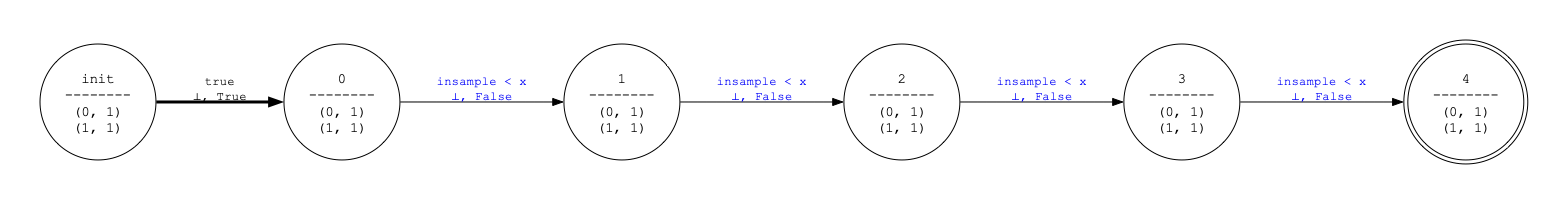
\includegraphics[width=0.9\textwidth]{figures/only_l_transitions.png}
        \caption{A segment $s$ with only L-transitions.}
        \label{fig:segment_j}
    \end{figure}

    \begin{figure}[H]
        \centering
        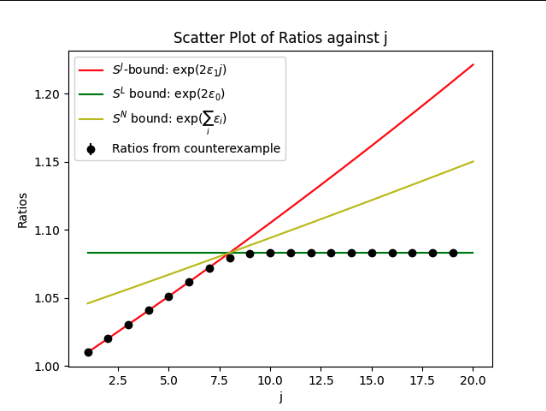
\includegraphics[width=0.5\textwidth]{figures/only_l_transitions_plot.png}
        \caption{}
        \label{fig:segment_j_coupling}
    \end{figure}
\end{proof}

\begin{hypothesis}
    For segments which contain only $L$-transitions and for which the $J$-cost exceeds the $L$-cost, $S^L$ is tight.
\end{hypothesis}

\begin{proof}
    I think this is true from the graph above, but I need to prove it.

    Note June 28 2023: I think this is not true for segments that contain both $L$-transitions and $G$-transitions.
\end{proof}

\appendix

\section{Lemmata}

\subsection{Properties of $f_\epsilon$ and $F_\epsilon$}

\begin{lemma} 
    \label{lemma:F_equality_neg}
    For $x \leq 0$, we have 
    \[F_\epsilon(x) = \exp(2\epsilon)F_\epsilon(x - 2)\]
    and equivalently for $x \leq -2$, we have 
    \[F_\epsilon(x + 2) = \exp(2\epsilon)F_\epsilon(x)\]
\end{lemma}

\begin{lemma}
    \label{lemma:F_equality_pos}
    For $x \geq 0$, we have \[1 - F_{\epsilon}(x) = \exp(2\epsilon) (1 - F_\epsilon(x + 2))\]
\end{lemma}

\begin{lemma}
    \label{lemma:f_equality}
    For $x \geq 0$, we have
    \[f_\epsilon(x) = \exp(2\epsilon) f_\epsilon(x + 2) \]
\end{lemma}

\subsection{For the proof of Theorem 1}
\begin{lemma} 
    \label{lemma:sl_tight_minus_infty} 
    \[\int_{-\infty}^{-2} f_{\epsilon}(x) F_{\epsilon}(x + 2)^\ell (1 - F_{\epsilon}(x))^m \dif x = \exp(2 \epsilon \ell) \int_{-\infty}^{-2} f_{\epsilon}(x) F_{\epsilon}(x)^\ell (1 - F_{\epsilon}(x))^m \dif x\]
\end{lemma}

\begin{proof}
    From Lemma \ref{lemma:F_equality_neg}, we have that 

    \begin{align*}
        \int_{-\infty}^{-2} f_{\epsilon}(x) F_{\epsilon}(x + 2)^\ell (1 - F_{\epsilon}(x))^m \dif x &= \int_{-\infty}^{-2} f_{\epsilon}(x) (\exp(2\epsilon) F_{\epsilon}(x))^\ell (1 - F_{\epsilon}(x))^m \dif x \\
        &= \exp(2\epsilon \ell) \int_{-\infty}^{-2} f_{\epsilon}(x) F_{\epsilon}(x)^\ell (1 - F_{\epsilon}(x))^m \dif x
    \end{align*}
\end{proof}

\begin{lemma}
    \label{lemma:sl_tight_plus_infty}
    \[\int_{0}^{\infty} f_{\epsilon}(x) F_{\epsilon}(x + 2)^\ell (1 - F_{\epsilon}(x))^m \dif x = \exp(2 \epsilon m) \int_{2}^{\infty} f_{\epsilon}(x) F_{\epsilon}(x)^\ell (1 - F_{\epsilon}(x))^m \dif x\]
\end{lemma}

\begin{proof}
    From Lemma \ref{lemma:F_equality_pos} and \ref{lemma:f_equality}, we have that

    \begin{align*}
        \int_{0}^{\infty} f_{\epsilon}(x) F_{\epsilon}(x + 2)^\ell (1 - F_{\epsilon}(x))^m \dif x &= \int_{0}^{\infty} \exp(2\epsilon)f_{\epsilon}(x + 2) F_{\epsilon}(x + 2)^\ell (\exp(2\epsilon)(1 - F_{\epsilon}(x + 2)))^m \dif x \\
        &= \exp(2\epsilon m) \int_{0}^{\infty} f_{\epsilon}(x + 2) F_{\epsilon}(x + 2)^\ell (1 - F_{\epsilon}(x + 2))^m \dif x\\
        &= \exp(2\epsilon (m + 1)) \int_{2}^{\infty} f_{\epsilon}(x) F_{\epsilon}(x)^\ell (1 - F_{\epsilon}(x))^m \dif x
    \end{align*}
\end{proof}

\begin{lemma}
    There exists a function $g: \N \to \mathbb{R}$ such that
    \label{lemma:sl_tight_minus_2}
    \[\int_{-2}^{0} f_{\epsilon}(x) F_{\epsilon}(x + 2)^\ell (1 - F_{\epsilon}(x))^m \dif x = g(\ell) \exp(2 \epsilon (m + 1)) \int_{-2}^{2} f_{\epsilon}(x) F_{\epsilon}(x)^\ell (1 - F_{\epsilon}(x))^m \dif x\]
    with $g(\ell) \to 1$ as $\ell \to \infty$.
\end{lemma}

\begin{proof}
    I'm not sure yet how to prove this, although I strongly suspect that the $(m + 1)$ term comes from the fact that $f_{\epsilon}(x)$ is the derivative of $-(1 - F_{\epsilon}(x))$, and it is taken to the $m$th power. Its integral should behave like a polynomial of degree $m + 1$ evaluated at $2$, which corresponds to $\exp(2\epsilon(m + 1))$. 
\end{proof}


\end{document}